\section{Python : origine et philosophie}
\subsection{L'origine de Python}
\begin{frame}
  \frametitle{L'origine de Python}
  \begin{columns}
    \begin{column}{5cm}
      \begin{itemize}
        \item<1-> Apparition en 1991
        \item<2-> Créé par Guido van Rossum
        \item<3-> Nombreuses références aux Monty Python
      \end{itemize}
    \end{column}
    \begin{column}{5cm}
      \begin{overprint}
        \includegraphics<2>[scale=0.04]{guido.jpg}
        \includegraphics<3>[scale=0.15]{spam.jpg}
      \end{overprint}
    \end{column}
  \end{columns}
\end{frame}

\subsection{Valeurs et philosophie}
\begin{frame}
\frametitle{Valeurs et philosophie}
  \begin{itemize}
    \item Orienté objet
    //note feth:
    //utilisation souple (programmation impérative, orientée aspect, haut niveau ou bas niveau...)
    \pause
    \item Extensible (librairies standard, modules C, C++, ...)
  \end{itemize}
\end{frame}

\subsection{La recherche du meilleur chemin}
\begin{frame}
\frametitle{La recherche du meilleur chemin}
  \begin{itemize}
    \item Un travail de recherche via les PEP
    \pause
    //note feth:
    //mots clefs: efficacité en terme de lisibilité, pythonique, élégance (comme en maths)
    \item 1 seul bon moyen de faire
  \end{itemize}
\end{frame}



\section{IPython, le Python interactif}
\subsection{Les fonctionnalités}

\begin{frame}
  \frametitle{Fonctionnalités}
  \begin{itemize}
    \item Exécution de code dynamique
    \item Interaction avec le système
    \item Historique des commandes
    \item Journalisation
  \end{itemize}
\end{frame}

\subsection{Utile pour ...}
\begin{frame}[fragile]
  \frametitle{Utile pour ...}
    \begin{itemize}
      \item apprendre la syntaxe
    \end{itemize}
  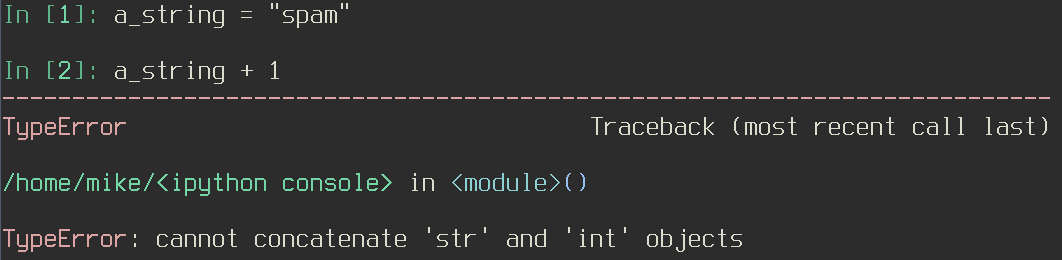
\includegraphics[scale=0.35]{apprendre.png}

\end{frame}

\begin{frame}
  \frametitle{Utile pour ...}
    \begin{itemize}
      \item prototyper une fonctionnalité
    \end{itemize}
    //note feth:
    // 1)
    //plutôt qu'un getter sur une var publique
    //je suggère une fonction qui fasse quelque chose, comme
    //def greet(self, name):
    //    return "%s greets %s." (self.name, name)
    // à votre avis ?
    //
    // 2) mentionner le ducktyping ? (à votre avis)
  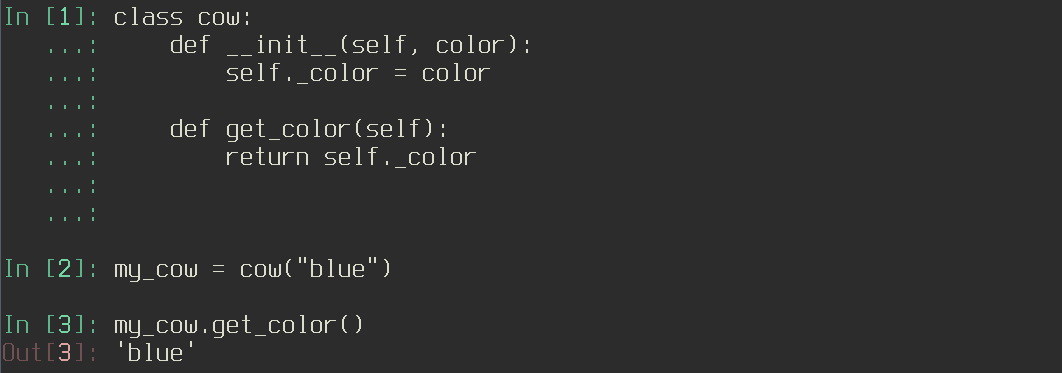
\includegraphics[scale=0.35]{prototype.png}
\end{frame}

\begin{frame}
  \frametitle{Utile pour ...}
    \begin{itemize}
      \item la découverte interactive d'une API
    \end{itemize}
  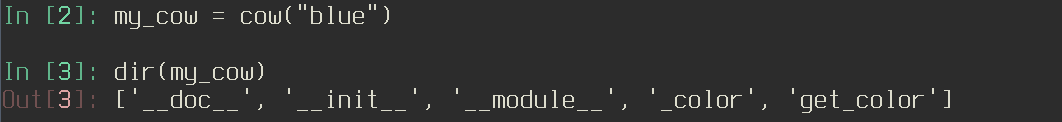
\includegraphics[scale=0.35]{api_discover.png}
\end{frame}

\begin{frame}
  \frametitle{Utile pour ...}
    \begin{itemize}
      \item embarquer un shell IPython dans ses programmes
    \end{itemize}
  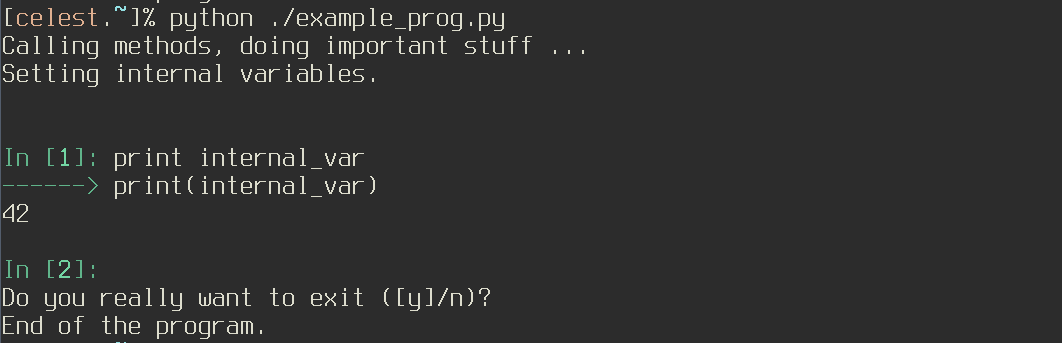
\includegraphics[scale=0.35]{embedded_ipython.png}
\end{frame}

\section{La syntaxe Python}
\subsection{Les principaux types de structure}

\begin{frame}
  \frametitle{Les principaux types de structure}
    \begin{itemize}
      \item<1-> les entiers
      \item<2-> les chaînes de caractère
      \item<3-> les tuples
      \item<4-> les listes
      \item<5-> les sets
      \item<6-> les dictionnaires
      \item<7-> les booléens
      //note feth: la valeur 'Rien' plutôt.
      // None est un objet singleton très pratique qu'on peut manipuler et qui a des attributs, contrairement à NULL, pointeur vers 0x0 (on ne parle pas de pointeurs en Python).
      // à votre avis ?
      \item<8-> la valeur nulle
    \end{itemize}
\end{frame}

\begin{frame}
  \frametitle{Les principaux types de structure ...}
    \begin{itemize}
      \item les entiers
    \end{itemize}
    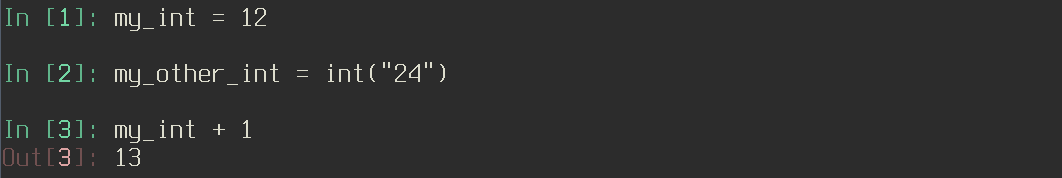
\includegraphics[scale=0.35]{type_int.png}
\end{frame}

\begin{frame}
  \frametitle{Les principaux types de structure ...}
    \begin{itemize}
      \item les chaînes de caractères
    \end{itemize}
    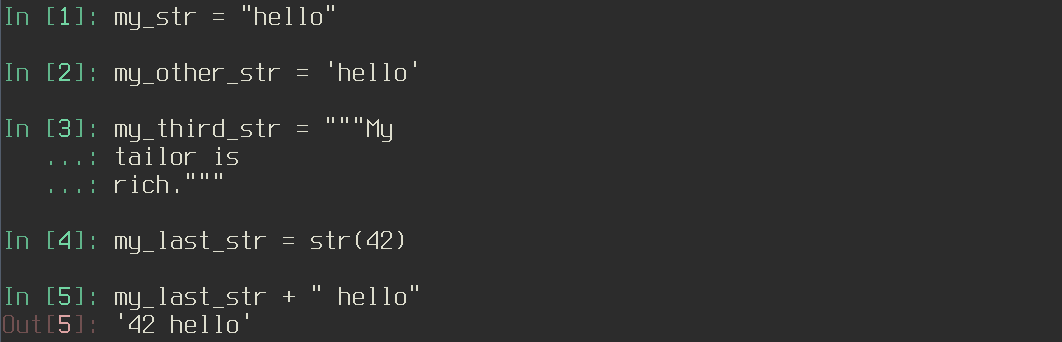
\includegraphics[scale=0.35]{type_str.png}
\end{frame}

\begin{frame}
  \frametitle{Les principaux types de structure ...}
    \begin{itemize}
      \item les tuples
    \end{itemize}
    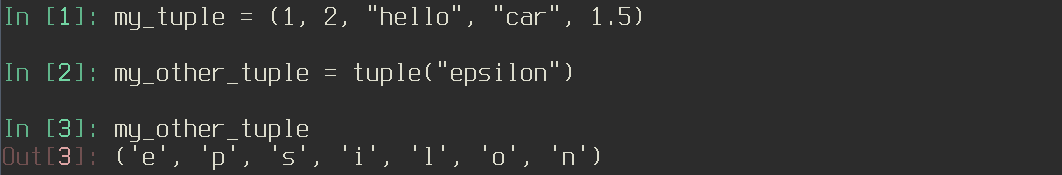
\includegraphics[scale=0.35]{type_tuple.png}
\end{frame}

\begin{frame}
  \frametitle{Les principaux types de structure ...}
    \begin{itemize}
      \item les listes
    \end{itemize}
    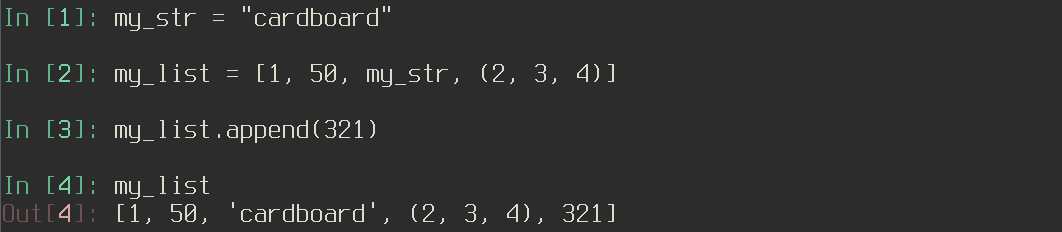
\includegraphics[scale=0.35]{type_list.png}
\end{frame}

\begin{frame}
  \frametitle{Les principaux types de structure ...}
    \begin{itemize}
      \item les sets
    \end{itemize}
    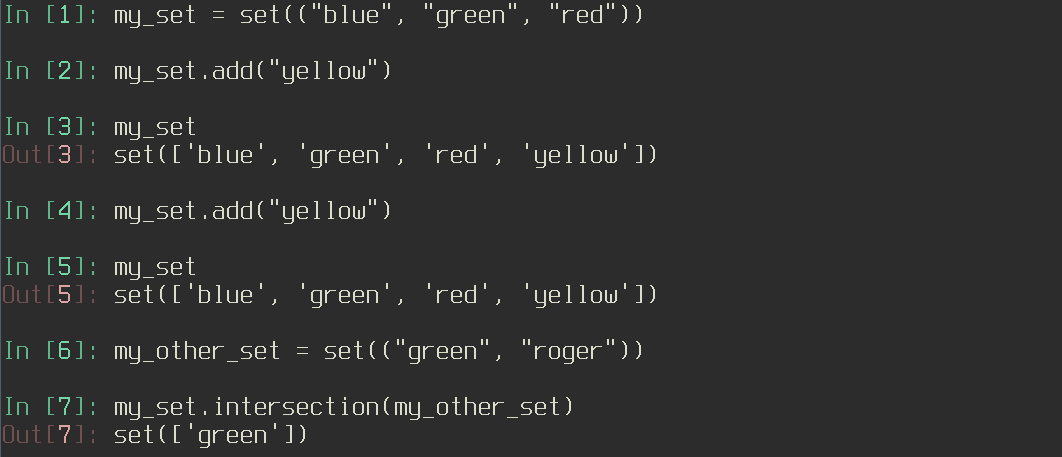
\includegraphics[scale=0.35]{type_set.png}
\end{frame}

\begin{frame}
  \frametitle{Les principaux types de structure ...}
    \begin{itemize}
      \item les dictionnaires
    \end{itemize}
    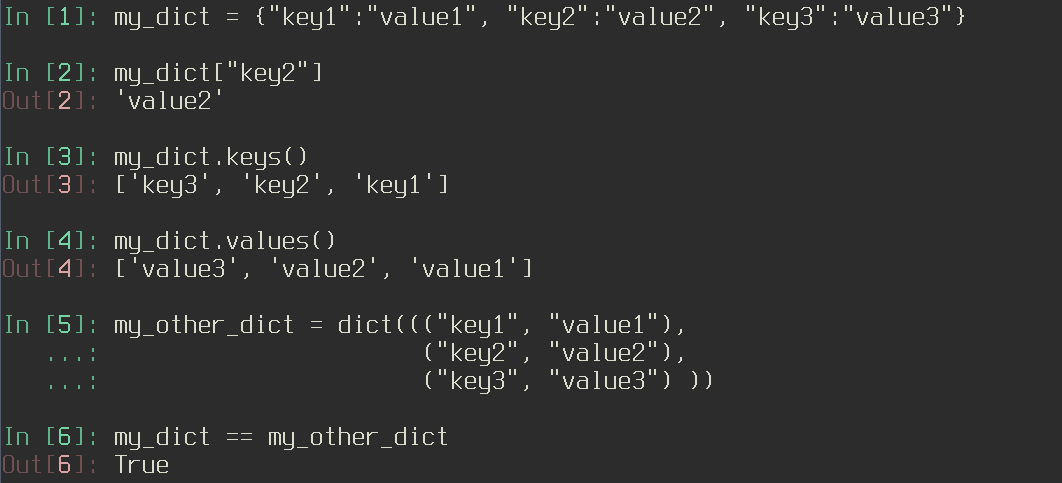
\includegraphics[scale=0.35]{type_dict.png}
\end{frame}

\begin{frame}
  \frametitle{Les principaux types de structure ...}
    \begin{itemize}
      \item les booléens : True, False
      \item la valeur nulle : None
    \end{itemize}
\end{frame}

\subsection{Les déclarations conditionnelles}
\begin{frame}[fragile]
  \frametitle{Syntaxe de base}
  \begin{lstlisting}
if condition1:
    declaration1
elif condition2:
    declaration2
else:
    declaration3
  \end{lstlisting}
\end{frame}

\begin{frame}[fragile]
  \frametitle{Structure de base - exemple}
  \begin{lstlisting}
my_str = "word"
if 1 > 2:
    print "1>2"
elif my_str == "word":
    print "my_str = word"
else:
    print "else"
  \end{lstlisting}

  \begin{beamercolorbox}{terminal}
  \begin{semiverbatim}
 \$ python example.py
 \uncover<2>{my_str = word} \end{semiverbatim}
  \end{beamercolorbox}

\end{frame}

\begin{frame}[fragile]
  \frametitle{Les conditions}
  \begin{itemize}
    \item les comparaisons
  \end{itemize}
  \begin{beamercolorbox}{terminal}
  \begin{semiverbatim}
\uncover<1->{ In [1]: (1 == 2, 1 < 2, 2 < 1, 1 != 2)}
\uncover<1->{ Out[1]: (False, True, False, True)}

\uncover<2>{ In [2]: my_str = "hello"}
\uncover<2>{ In [2]: (my_str == "hello", my_str > "helln",
    ...: my_str < "hellq")}
\uncover<2>{ Out[2]: (True, True, True)}\end{semiverbatim}
    \end{beamercolorbox}
\end{frame}

\begin{frame}[fragile]
  \frametitle{Les conditions}
  \begin{itemize}
    \item les opérateurs booléens
  \end{itemize}
  \begin{beamercolorbox}{terminal}
  \begin{semiverbatim}
 In [1]: not True and False or not False
 Out[1]: True\end{semiverbatim}
  \end{beamercolorbox}
\end{frame}

\begin{frame}[fragile]
  \frametitle{Les conditions}
  \begin{itemize}
    \item par extension, certains objets vides sont équivalent à False
  \end{itemize}
  \begin{beamercolorbox}{terminal}
  \begin{semiverbatim}
 In [1]: my_str = ""
 In [1]: if not my_str:
    ...:     print "False"
 False\end{semiverbatim}
  \end{beamercolorbox}
\end{frame}

\subsection{Les boucles}
\begin{frame}[fragile]
  \frametitle{Syntaxe de for}
  \begin{lstlisting}
for item in <generator>:
    code ...
  \end{lstlisting}
\end{frame}

\subsection{Les méthodes/functions}
\begin{frame}[fragile]
\end{frame}

\subsection{Les classes}
\begin{frame}[fragile]
\end{frame}

\section{Quelques librairies standard}
\begin{frame}[fragile]
\end{frame}

%  \framesubtitle{The proof uses \textit{reductio ad absurdum}.}
%  \begin{theorem}
%      There is no largest prime number.
%  \end{theorem}
%  \begin{proof}
%    \begin{enumerate}
%      \item<1-| alert@1> Suppose $p$ were the largest prime number.
%      \item<2-> Let $q$ be the product of the first $p$ numbers.
%      \item<3-> Then $q+1$ is not divisible by any of them.
%      \item<1-> Thus $q+1$ is also prime and greater than $p$.\qedhere
%    \end{enumerate}
%  \end{proof}

%\setbeamercolor{terminal}{fg=white, bg=black}
%\begin{beamercolorbox}{terminal}
%\end{beamercolorbox}
